\section{Battery Models}\label{sec:kibam}
Schedules for space missions need to be battery aware, in order for their satellite too function correctly and not fall out of their orbit or lose connection with the satellite. This part will focus on what battery model to use in CORA and subsuquently for SMC. As mentioned previous CORA does not allow differential equations in their models, which has to be taking into account when chosen the battery model.

Batteries are complicated to simulate due to its chemical properties, and the different kinds of batteries makes is it even worse. One thing all batteries have in common is the ability to store chemical energy and convert it into electricity. But another factor like recovery effect dependents on the type of battery and can have large impact on the expected lifetime, recovery effect happen after battery has been discharged for a period, the amount of current applied to the battery effects the recovery effect. The performance of the different models will be compared to the actual measured of a lithium-ion battery, measured are taken from \cite{battery_lifetime_analysis}.

The Ideal model is very simplistic due to it only taking two variables to determine the batteries lifetime(L), capacity(C) and load current(I). Capacity refereed to the batteries amount of amp-hours, and load current is the constant discharge on the battery in amps. The formal for this is shown in \cref{eq:bm}.

\begin{equation}\label{eq:bm}
L=C/I
\end{equation}

Performance of the Ideal model can be seen in \cref{table:t-Ideal}. The table is divided into two parts, constant load and variable load, the column ``Measured, min'' show the actual reading of the lithium-ion battery under the different loads. To the right the Ideal estimation are shown. In general the Ideal model overestime the expected lifetime in all cases, shown in T1 the diviation from the actual measures differes by 28.58\%, a trend seems to appear in that lower amps often results in better predictions from the Ideal model with constant loads. Only T5 and T6 dose not apply to this, because T5 have a better prediction then T6 even though T5 has a higher load. During variable loads all cases overestimate by a substantial amount, the closes approximation is C5 with a 18.5\% overestimation. The data shows that the Ideal model does a poor job of estimating the actual lifetime of a battery, which is properly because the Ideal model asumes linear effcet for lifetime estimation. Additionally for variables loads the Ideal model does not consider recovery effect of the battery which further misses the measured minutes. 

% Please add the following required packages to your document preamble:
% \usepackage[table,xcdraw]{xcolor}
% If you use beamer only pass "xcolor=table" option, i.e. \documentclass[xcolor=table]{beamer}
\begin{table}[]
	\centering
	\scalebox{0.8}{
	\begin{tabular}{|llllll|lllll|}
		\hline
		\multicolumn{6}{|c|}{Constant load} & \multicolumn{5}{c|}{Variable load} \\ \hline
		\rowcolor[HTML]{EFEFEF} 
		\multicolumn{1}{|l|}{\cellcolor[HTML]{EFEFEF}Test} & \multicolumn{1}{l|}{\cellcolor[HTML]{EFEFEF}I, amps} & \multicolumn{1}{l|}{\cellcolor[HTML]{EFEFEF}Measured, min} & \multicolumn{1}{l|}{\cellcolor[HTML]{EFEFEF}Ideal, min} & \multicolumn{1}{l|}{\cellcolor[HTML]{EFEFEF}$\Delta$T} & \%$\Delta$ & \multicolumn{1}{l|}{\cellcolor[HTML]{EFEFEF}Test} & \multicolumn{1}{l|}{\cellcolor[HTML]{EFEFEF}Measured, min} & \multicolumn{1}{l|}{\cellcolor[HTML]{EFEFEF}Ideal, min} & \multicolumn{1}{l|}{\cellcolor[HTML]{EFEFEF}$\Delta$C} & \%$\Delta$ \\ \hline
		T1 & 222.7 & 141.0 & 181.3 & 40.3 & 28.58\% & C1 & 54.5 & 70.8 & 16.3 & 29.91\% \\ \hline
		\rowcolor[HTML]{EFEFEF} 
		T2 & 204.5 & 156.6 & 197.4 & 40.8 & 26.05\% & C2 & 73.3 & 91.9 & 18.6 & 25.38\% \\ \hline
		T3 & 108.3 & 307.8 & 372.8 & 65 & 21.12\% & C3 & 88.3 & 108.5 & 20.2 & 22.88\% \\ \hline
		\rowcolor[HTML]{EFEFEF} 
		T4 & 107.5 & 312.0 & 375.6 & 63.6 & 20.38\% & C4 & 136.0 & 163.0 & 27 & 19.85\% \\ \hline
		T5 & 94.9 & 358.2 & 425.4 & 67.2 & 18.76\% & C5 & 182.7 & 216.5 & 33.8 & 18.50\% \\ \hline
		\rowcolor[HTML]{EFEFEF} 
		T6 & 84.3 & 397.2 & 478.9 & 81.7 & 20.57\% & C6 & 59.0 & 74.7 & 15.7 & 26.61\% \\ \hline
		T7 & 75.5 & 448.2 & 534.8 & 86.6 & 19.32\% & C7 & 51.1 & 66.9 & 15.8 & 30.92\% \\ \hline
		\rowcolor[HTML]{EFEFEF} 
		T8 & 28.0 & 1248 & 1442 & 194 & 15.54\% & C8 & 55.0 & 70.8 & 15.8 & 28.73\% \\ \hline
		T9 & 19.5 & 1818 & 2071 & 253 & 13.92\% & C9 & 54.9 & 70.8 & 15.9 & 28.96\% \\ \hline
		\rowcolor[HTML]{EFEFEF} 
		T10 & 3.0 & 12690 & 13458 & 768 & 6.05\% & C10 & 142.7 & 171.3 & 28.6 & 20.04\% \\ \hline
	\end{tabular}}
	\caption{Comparison of Actual measure against Ideal model. Ideal data taken from \cite{battery_model}. Specification for the variable loads can be found in \cref{variable_loads_list}
	}
	\label{table:t-Ideal}
\end{table}

Peukert Model introduces a few new variables in comparison to the Ideal model, like the previous we still want to estimate the expected lifetime, but to better represent the battery a non-linear model is needed. Peukert fixes this by introducing two new variables: discharge time(H) and Peukert Exponent(k), the formal can be see in \cref{eq:pm}. Both values k and h is special in the sense that it is only observerable through examiniation of the battery, this is typically done by the manufactor. H is the discharge time in hours and k is an exponent often be provided by the battery manufactors.
\begin{equation}\label{eq:pm}
L=H(\frac{C}{IH})^k
\end{equation}
\begin{itemize}
	\item L - lifetime in hours
	\item H - discharge time in hours based on amp hours(AH)
	\item C - capacity in AH
	\item I - load current in amps
	\item k - Peukert Exponent
\end{itemize}

\cref{table:t-Peukert} showcases the estimations using Peukert. In most cases Peukert overestimate except for one instance in test T10, it underestimate with 3.17\%. It seems to become more accruate the smaller the amps are, with the outliner, T5 and T6 Similarly to \cref{table:t-Ideal}. One thing to notices is that for variable loads it still has a high mismatch compared to measured values, this is due to Peukerts model not taken recovery effect into account. But overall Peukert performance better than the Ideal model.

\begin{table}[]
	\centering
	\scalebox{0.8}{
	\begin{tabular}{|llllll|lllll|}
\hline
\multicolumn{6}{|c|}{Constant load} & \multicolumn{5}{c|}{Variable load} \\ \hline
\rowcolor[HTML]{EFEFEF} 
\multicolumn{1}{|l|}{\cellcolor[HTML]{EFEFEF}Test} & \multicolumn{1}{l|}{\cellcolor[HTML]{EFEFEF}I, amps} & \multicolumn{1}{l|}{\cellcolor[HTML]{EFEFEF}Measured, min} & \multicolumn{1}{l|}{\cellcolor[HTML]{EFEFEF}Peukert, min} & \multicolumn{1}{l|}{\cellcolor[HTML]{EFEFEF}$\Delta$T} & \%$\Delta$ & \multicolumn{1}{l|}{\cellcolor[HTML]{EFEFEF}Test} & \multicolumn{1}{l|}{\cellcolor[HTML]{EFEFEF}Measured, min} & \multicolumn{1}{l|}{\cellcolor[HTML]{EFEFEF}Peukert, min} & \multicolumn{1}{l|}{\cellcolor[HTML]{EFEFEF}$\Delta$C} & \%$\Delta$ \\ \hline
T1 & 222.7 & 141.0 & 154.5 & 13.5 & 9.57\% & C1 & 54.5 & 60.5 & 6 & 11.01\% \\ \hline
\rowcolor[HTML]{EFEFEF} 
T2 & 204.5 & 156.6 & 168.4 & 11.8 & 7.54\% & C2 & 73.3 & 79.1 & 5.8 & 7.91\% \\ \hline
T3 & 108.3 & 307.8 & 321.3 & 13.5 & 4.39\% & C3 & 88.3 & 93.8 & 5.5 & 6.23\% \\ \hline
\rowcolor[HTML]{EFEFEF} 
T4 & 107.5 & 312.0 & 323.7 & 11.7 & 3.75\% & C4 & 136.0 & 142.5 & 6.5 & 4.78\% \\ \hline
T5 & 94.9 & 358.2 & 367.5 & 9.3 & 2.60\% & C5 & 182.7 & 190.2 & 7.5 & 4.11\% \\ \hline
\rowcolor[HTML]{EFEFEF} 
T6 & 84.3 & 397.2 & 414.4 & 17.2 & 4.33\% & C6 & 59.0 & 64.4 & 5.4 & 9.15\% \\ \hline
T7 & 75.5 & 448.2 & 463.6 & 15.4 & 3.44\% & C7 & 51.1 & 56.5 & 5.4 & 10.57\% \\ \hline
\rowcolor[HTML]{EFEFEF} 
T8 & 28.0 & 1248 & 1270 & 22 & 1.76\% & C8 & 55.0 & 60.5 & 5.5 & 10.00\% \\ \hline
T9 & 19.5 & 1818 & 1835 & 17 & 0.94\% & C9 & 54.9 & 60.5 & 5.6 & 10.20\% \\ \hline
\rowcolor[HTML]{EFEFEF} 
T10 & 3.0 & 12690 & 12288 & -402 & -3.17\% & C10 & 142.7 & 148.8 & 6.1 & 4.27\% \\ \hline
\end{tabular}}
	\caption{Comparison of Actual measure against Peukert model. Peukert data taken from \cite{battery_model}. Specification for the variable loads can be found in \cref{variable_loads_list}
	}
	\label{table:t-Peukert}
\end{table}

\gls{kibam} uses two wells as an abstract concept to represent a battery. It consist of an available charge and a bound charge as shown in \cref{fig:kibam_wells}, c dertermines the ratio of the two wells based on the total capacity. Current can only be drawn from the available charge, when the available charges height $h_2$ is lower then bound charge height $h_1$, charge start o flow from bound charge to available charge until both wells are at equal height. The rate of this flow is determinded by the value k, this simulate the recovery effect of the battery like previous models was not able to capture. To calculate $y{1}$ and $y{2}$ can be seen in \cref{eq:y1} and\cref{eq:y2} along with a short description of the variables used in these equations. 

\begin{figure}
	\center
	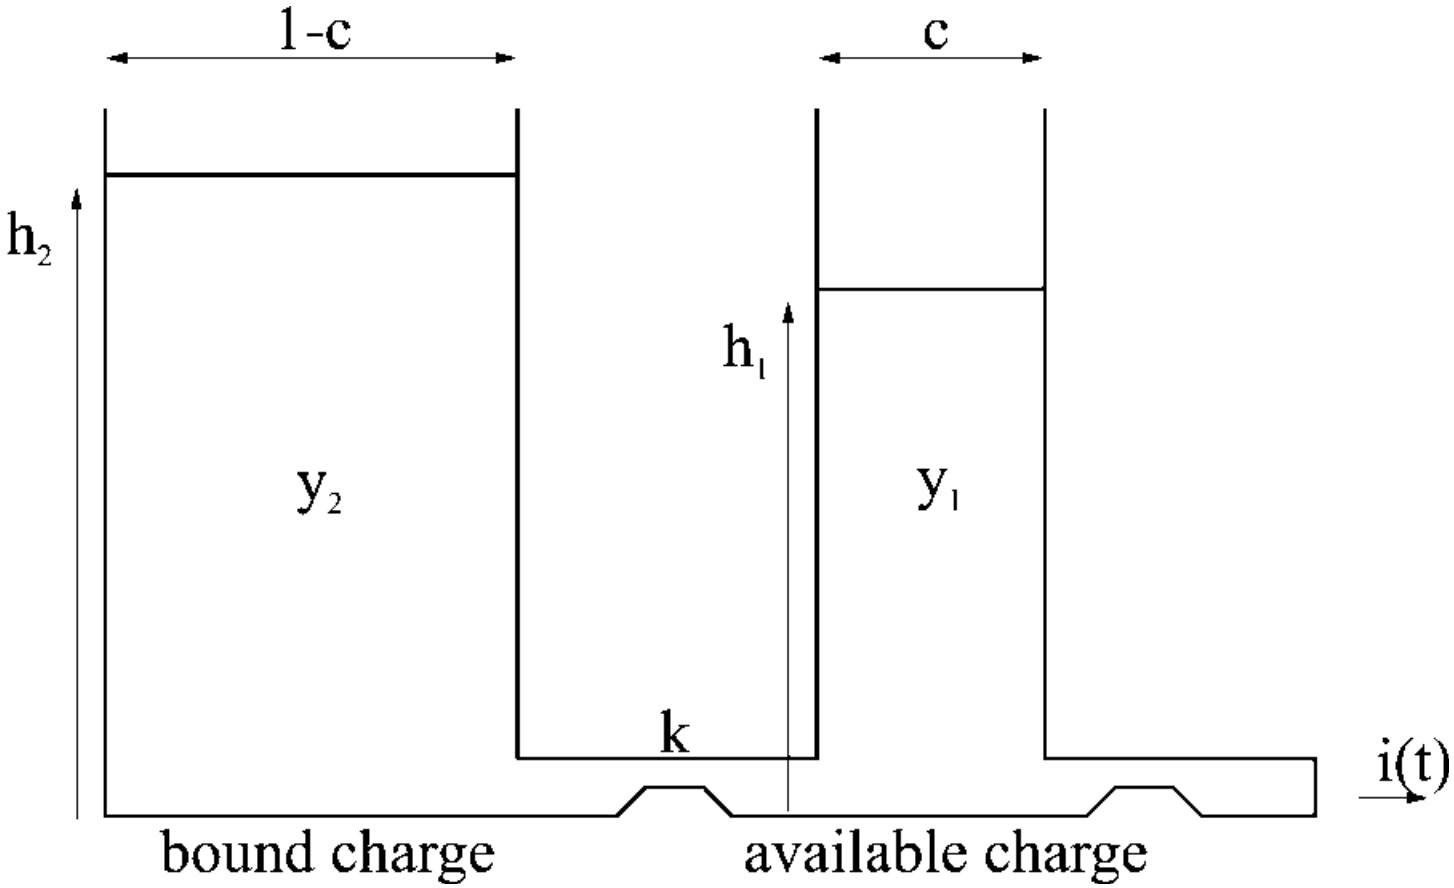
\includegraphics[width=\textwidth/2]{graphics/kibam.jpg}
	\label{fig:kibam_wells}
	\caption{Displays the two wells of \gls{kibam}}
\end{figure}

\begin{equation}\label{eq:y1}
y_1(t) = cCe^{-k't}+\frac{(y_0k'c-I)(1-e^{-k't})}{k'}-\frac{Ic(k't-1+e^{-k't})}{k'}
\end{equation}

\begin{equation}\label{eq:y2}
y_2(t) = (1-c)Ce^{-k't}+y_0(1-c)(1-e^{-k't})-\frac{I(1-c)(k't-1+e^{-k't})}{k'}
\end{equation}

Short description of the variables used in th
C = capacity in AH
e = euler's number
k' = k/c(1-c)
k = defined value
t = time in hours
c = ratio between available and bound charge
I = load also refered to as current applyed on the battery

Performance of \gls{kibam} can be seen in \cref{table:t-KiBaM}. Under constant load the results vary, and he only indicating is that an amps above 110 and below 20 seems to give better results. Interesting for variable loads is that all of the predictions from \gls{kibam} underestimate compared to the measured values, some are fairly high though, like in case C7 it underestimate by 40.31\%.  

\begin{table}[]
	\centering
	\scalebox{0.8}{
	\begin{tabular}{|l|lllll|llll|l|}
\hline
\multicolumn{6}{|c|}{Constant load} & \multicolumn{5}{c|}{Variable load} \\ \hline
\rowcolor[HTML]{EFEFEF} 
Test & \multicolumn{1}{l|}{\cellcolor[HTML]{EFEFEF}I, amps} & \multicolumn{1}{l|}{\cellcolor[HTML]{EFEFEF}Measured, min} & \multicolumn{1}{l|}{\cellcolor[HTML]{EFEFEF}KiBaM, min} & \multicolumn{1}{l|}{\cellcolor[HTML]{EFEFEF}$\Delta$T} & \%$\Delta$ & \multicolumn{1}{l|}{\cellcolor[HTML]{EFEFEF}Test} & \multicolumn{1}{l|}{\cellcolor[HTML]{EFEFEF}Measured, min} & \multicolumn{1}{l|}{\cellcolor[HTML]{EFEFEF}KiBaM, min} & $\Delta$T & \%$\Delta$ \\ \hline
T1 & 222.7 & 141.0 & 139.9 & -1.1 & -0.78\% & C1 & 54.5 & 36.3 & -18.2 & -33.39\% \\ \hline
\rowcolor[HTML]{EFEFEF} 
T2 & 204.5 & 156.6 & 156 & -0.6 & -0.38\% & C2 & 73.3 & 55.7 & -17.6 & -24.01\% \\ \hline
T3 & 108.3 & 307.8 & 331.4 & 23.6 & 7.67\% & C3 & 88.3 & 71.4 & -16.9 & -19.14\% \\ \hline
\rowcolor[HTML]{EFEFEF} 
T4 & 107.5 & 312.0 & 334.1 & 22.1 & 7.08\% & C4 & 136.0 & 123.6 & -12.4 & -9.12\% \\ \hline
T5 & 94.9 & 358.2 & 384 & 25.8 & 7.20\% & C5 & 182.7 & 175.7 & -7 & -3.83\% \\ \hline
\rowcolor[HTML]{EFEFEF} 
T6 & 84.3 & 397.2 & 437.5 & 40.3 & 10.15\% & C6 & 59.0 & 41.1 & -17.9 & -30.34\% \\ \hline
T7 & 75.5 & 448.2 & 493.3 & 45.1 & 10.06\% & C7 & 51.1 & 30.5 & -20.6 & -40.31\% \\ \hline
\rowcolor[HTML]{EFEFEF} 
T8 & 28.0 & 1248 & 1401 & 153 & 12.26\% & C8 & 55.0 & 38.1 & -16.9 & -30.73\% \\ \hline
T9 & 19.5 & 1818 & 2029 & 211 & 11.61\% & C9 & 54.9 & 34.8 & -20.1 & -36.61\% \\ \hline
\rowcolor[HTML]{EFEFEF} 
T10 & 3.0 & 12690 & 13417 & 727 & 5.73\% & C10 & 142.7 & 131.7 & -11 & -7.71\% \\ \hline
\end{tabular}}
	\caption{Comparison of Actual measure against \gls{kibam} model. \gls{kibam} data taken from \cite{battery_model}. Specification for the variable loads can be found in \cref{variable_loads_list}
	}
	\label{table:t-KiBaM}
\end{table}

Looking at all the results for the three battery models, it show that Peukerts model give overall better estimation for variable loads then Ideal or \gls{kibam}. But the advandtage of using \gls{kibam} over Peukerts model under variable load is that \gls{kibam} always underestimate, which is good for our case, that ensure that we will never run into a case where the prediction cause the actual system to run out of energy. The Ideal is inferior to Peukerts and \gls{kibam} in almost all predictions, a summerize of the three differnent battry models can be found below.
\begin{itemize}
	\item Ideal model - linear representation of the battery with no support of recovery effect
	\item Peukert model - non-linear representation of the battery with no support of recovery effect
	\item \gls{kibam} - abstract representation of the battery with support of recovery effect
\end{itemize}
Since CORA can't use \gls{kibam}, Peukert model will be the second best options.

%Dualfoil model is based on the chemical proceses taking place in a battery, It is one of the most accruate models in the field. But the downside to this model is its complexity. It requires more than 50 parameters related to the battery properties to be set, and it uses six non-linear differential equations. Given the large set of parameters makes it difficult to configure corretly and in most cases often used purely as a comparison against other models.

%Diffusion model

%Eletrical-circuit Models, uses eletrical properties to model the battery. The most common properties to model in an eletrical-circuit model is capacity of the battery, lost capacity at high discharge currents, dischargeof battery, state of charge and battery's resistance. Compared to the eletrochemical models these are require overall less computational power to reprents the battery, but also less accruate.

%Stochastic models uses high level abstraction to represent the battery, one instance of this is with Marko chains where model has $N$ number of states, where N is the number of available charge units and it represent either the actual amount of amps or some arbetary amount like the amount of energy required to do an activity. Each time step there is a chance of remaining in the same state or going up one state or moving down one or several states, the battery is considered empty when state 0 is reached. For instance if a battery has 200 charge units, the battery will initialy start in state 200 given it is full, than after one time step the new possible range from 0 to 200, in this example we end in state 80.

%Analytical models also uses high level abstraction to capture the battery's properties.



%On the other end of the spectrum there is the most basic battery model that uses capacity(C) and load current(I) to calculate the lifetime(L) of a battery, given the formula 

%This asumes a constant load and the batteries properties are linear. 

%Modifing the basic battery model, we can capture the non-linear properties. This can be done with Peukert's law. 
%\begin{equation}
%L=H(\frac{C}{IH})^k
%\caption{Peukert's law Model}
%\end{equation}
%\begin{itemize}
%	\item L - lifetime in hours
%	\item H - discharge time in hours based on amp hours(AH)
%	\item C - capacity in AH
%	\item I - load current in amps
%	\item k - Peukert Exponent, often provided by manufacturs
%\end{itemize}
%http://all-about-lead-acid-batteries.capnfatz.com/all-about-lead-acid-batteries/lead-acid-battery-fundamentals/peukerts-law-and-exponent-explained/


%If we wan't to find out how long a 9 volt battery with 90AH can power a 200 watts, 120 volts light bulb. In \cref{BM:E1} the values have setup using the above information, the results show that it is possible to power a light blub for 53.9 hours. 

%\begin{equation}
%53.9=90/1.67
%\caption{Basic Model: 90AH battery powering light bulb}
%\label{BM:E1}
%\end{equation}
%\begin{equation}
%83.5656=18(\frac{90}{1.67*18})^1.4
%\caption{Peukert's law Model: 90AH battery powering light blub}
%\label{PLM:E1}
%\end{equation}

%More work on Stochastic models.


%Battery models plays an important part in schedules for space missions, and numerous models have been developed to capture how a battery functions in the real world. In the paper "what battery model to use?"\cite{battery_model} they go over the different types of battery models that exists, they analyse a wide range of models, where the electrochemical models being of the highest accuracy down to the most basic models. 
%Through the paper\cite{battery_model} they made some discoveries, first one being that the electrochemical models were often way to complex to be used in applications and was error prone if all setting were not set correctly. On the other side of the spectrum was the basic models which gave fairly good results, but under certain circumstances it would not perform well in respect to the real world battery. In between these two models are the analytical models, which seems to work well in any condition without high deviations. The analytical models introduced from the paper is KiBaM and diffusion model, they perform similarly. But the paper would suggest KiBaM to be used when modelling a battery, duo to it being more simplistic then the diffusion model \cite{battery_model}.
%use kibam in a stocastic setup to minimize error. 
%What battery model to use?

%KiBaM is an analytical model and uses an abstract model to represent the battery.